\stepcounter{slidesection}
\setbeamertemplate{background}[bgfirst]
\setbeamertemplate{footline}[first]
\subtitle{\theslidesection: Next Generation Sequencing}
% TODO
\titlegraphic{Kapitel/TechnischeGrundlagen/Bilder/logo2.png}
\begin{frame}[noframenumbering]
    \titlepage
    \begin{textblock}{10}(4.75,15)
        \cite{ProgrammingLogo}
    \end{textblock}
\end{frame}
\setbeamertemplate{footline}[presentationbody] 
\setbeamertemplate{background}[bgbody]

\begin{frame}{Geräte}
    \only<1->{
        \begin{textblock}{9.2}(1,3)
            \begin{mdframed}[backgroundcolor=white]
                \begin{center}
                    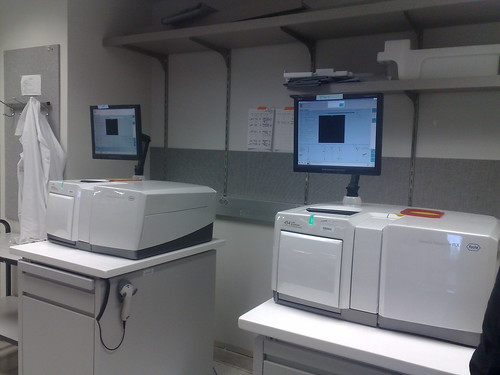
\includegraphics[height=5.2cm]{Kapitel/NGSTechnologien/Bilder/NGS454.jpg}\\
					\vspace{0.3cm}\captionof{figure}{Eins der ersten NGS-Geräte: Der Roche 454 (ca. 70k-700k Reads je 400-700 bp, bis ca. 500 Mbp)\cite{NGS454}}
                \end{center}
            \end{mdframed}
        \end{textblock}
    }
    \only<2->{
        \begin{textblock}{9.2}(2,3.1)
            \begin{mdframed}[backgroundcolor=white]
                \begin{center}
                    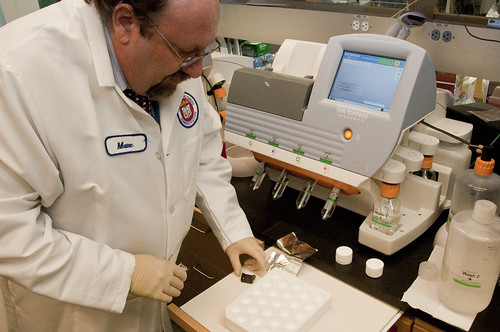
\includegraphics[height=5.2cm]{Kapitel/NGSTechnologien/Bilder/NGSPGM.jpg}\\
					\vspace{0.3cm}\captionof{figure}{Der spirituelle Nachfolger des 454: Der IonTorrent PGM (ca. 400k-4M Reads je 400 bp, bi ca. 1.6 Gbp)\cite{NGSPGM}}
                \end{center}
            \end{mdframed}
        \end{textblock}
    }
    \only<3->{
        \begin{textblock}{9.2}(3,3.2)
            \begin{mdframed}[backgroundcolor=white]
                \begin{center}
                    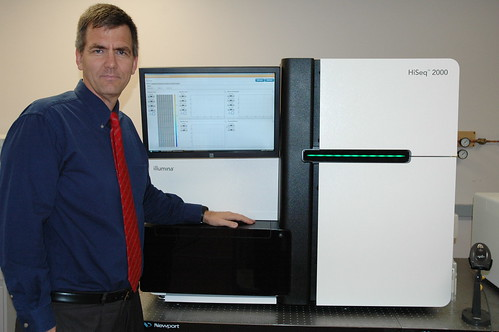
\includegraphics[height=5.2cm]{Kapitel/NGSTechnologien/Bilder/NGSHiSeq.jpg}\\
					\vspace{0.3cm}\captionof{figure}{Das Hauptgerät des aktuellen Marktführers: Ein Illumina HiSeq (ca. 2000M Reads je 250 bp, bis ca. 500 Gbp)\cite{NGSHiSeq}}
                \end{center}
            \end{mdframed}
        \end{textblock}
    }
    \only<4->{
        \begin{textblock}{9.2}(4,3.3)
            \begin{mdframed}[backgroundcolor=white]
                \begin{center}
                    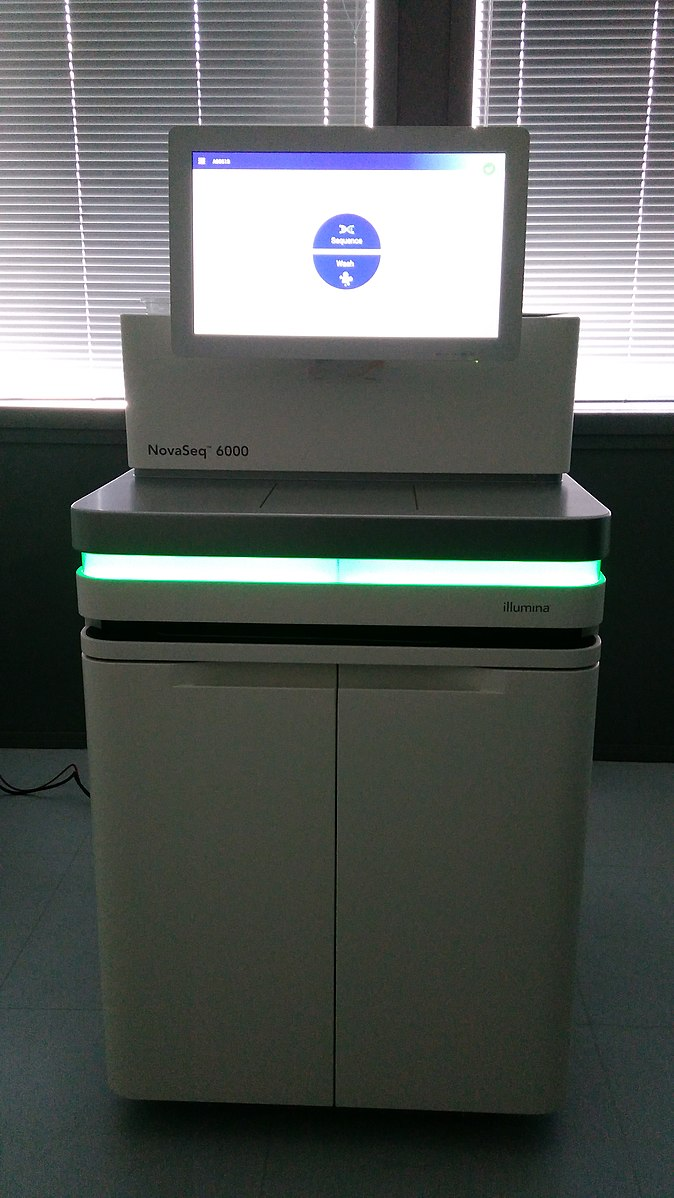
\includegraphics[height=5.2cm]{Kapitel/NGSTechnologien/Bilder/NGSNovaSeq.jpg}\\
					\vspace{0.3cm}\captionof{figure}{Das Großgerät des aktuellen Marktführers: Ein Illumina NovaSeq (ca. 10000M Reads je 300 bp, bis ca. 3 Tbp)\cite{NGSNovaSeq}}
                \end{center}
            \end{mdframed}
        \end{textblock}
    }
    \only<5->{
        \begin{textblock}{9.2}(5,3.4)
            \begin{mdframed}[backgroundcolor=white]
                \begin{center}
                    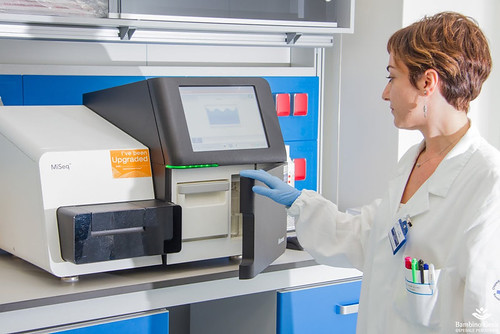
\includegraphics[height=5.2cm]{Kapitel/NGSTechnologien/Bilder/NGSMiSeq.jpg}\\
					\vspace{0.3cm}\captionof{figure}{Ein Kleingerät des aktuellen Marktführers: Ein Illumina MiSeq (ca. 25M Reads je 600 bp, bis ca. 15 Gbp)\cite{NGSMiSeq}}
                \end{center}
            \end{mdframed}
        \end{textblock}
    }
    \only<6->{
        \begin{textblock}{9.2}(6,3.5)
            \begin{mdframed}[backgroundcolor=white]
                \begin{center}
                    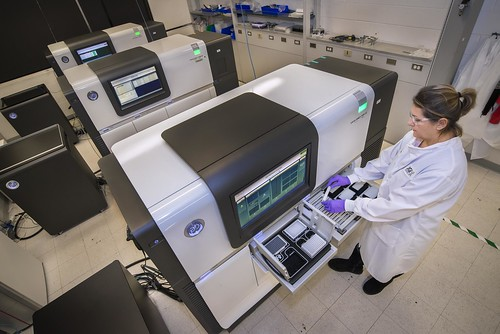
\includegraphics[height=5.2cm]{Kapitel/NGSTechnologien/Bilder/NGSPacBio.jpg}\\
					\vspace{0.3cm}\captionof{figure}{Großes 3rd Generation Sequencing-Gerät: Ein PacBio RSII (ca. 55K Reads je 15000 bp, bis ca. 900 Mbp)\cite{NGSPacBio}}
                \end{center}
            \end{mdframed}
        \end{textblock}
    }
    \only<7->{
        \begin{textblock}{9}(7,3.6)
            \begin{mdframed}[backgroundcolor=white]
                \begin{center}
                    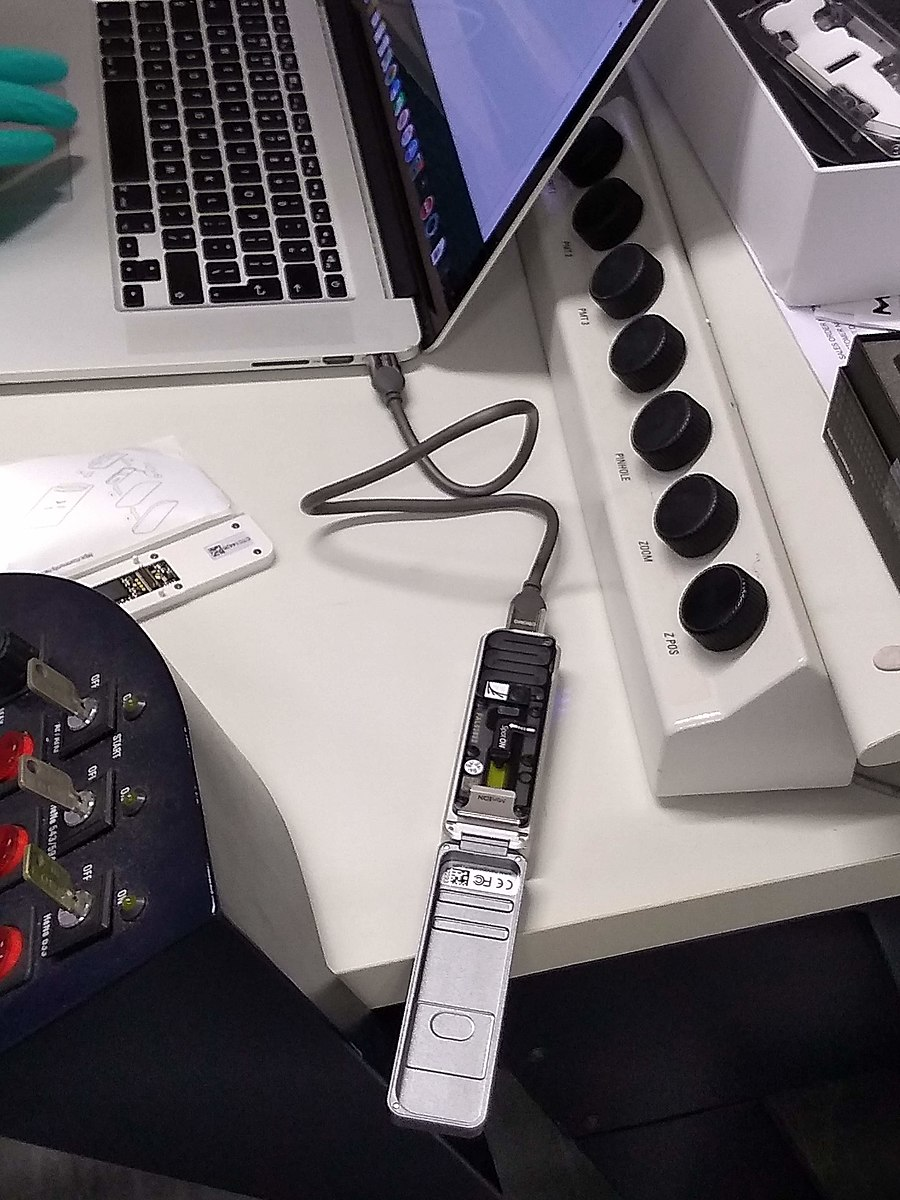
\includegraphics[height=5.2cm]{Kapitel/NGSTechnologien/Bilder/NGSMinION.jpg}\\
					\vspace{0.3cm}\captionof{figure}{Kleines 3rd Generation Sequencing-Gerät: Ein Oxford Nanopore MinION (bis zu 512 parallele Reads je bis ca. 2 Mbp, ca. 0.4 Mbp pro Stunde, bis ca. 50 Gbp)\cite{NGSMinION}}
                \end{center}
            \end{mdframed}
        \end{textblock}
    }
\end{frame}
